\section{Исследования}
\subsection{Тестовое множество}
\subsubsection{Изображения}
Для исследования были взяты изображения из открытой базы данных ImageNet, а так же из личной коллекции. Была произведенна следующая классификация:
\begin{itemize}
	\item Изображения людей
	\item Изображения архитектуры
	\item Изображения полученные при недостаточной освещенности
\end{itemize}
Данная классификация обусловлена распространенностью данных классов изображений и прикладных задачах в области обработки изображений. Фотографии людей используются как в повседневной жизни, так и во многих алгоритмах компьютерного зрения, таких как например распознавание лиц.

Не менее распространенны так же и изображения полученные при недостаточной освещенности, что приводит к низко контрастному изображению. Это мешает их анализу. Так же данные это актуально и для обычных пользователей фото и видеокамер, устройство которых все еще не позволяет достичь приемлимых результатов при съемке ночью. 

Последняя категория была выбрана в качестве примера, где  некоторые части изображения похожи друг на друга. Это может быть полезно в таких областях связанных с медициной, электроникой и астрономией. Где изображения, необходимы для последующей обработки имеют подобные свойства.

Ниже приведены примеры изображений из каждой категории.
\begin{figure}[H]
	\begin{center}
		\begin{minipage}[h]{0.5\linewidth}
			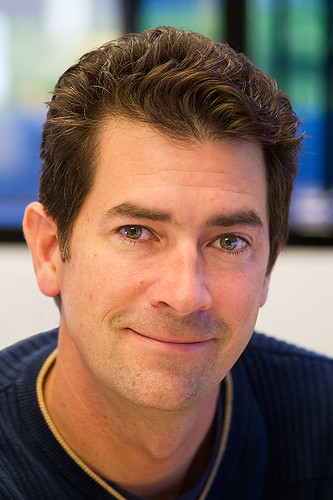
\includegraphics[draft]{imagePerson.png}
			\caption{Изобр. категории человек.} %% подпись к рисунку
			\label{img:imPerson} %% метка рисунка для ссылки на него
		\end{minipage}
		\hfill 
		\begin{minipage}[h]{0.5\linewidth}
			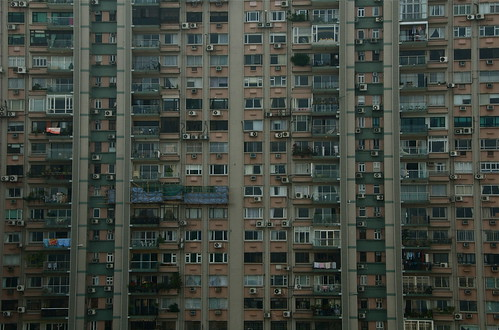
\includegraphics[draft]{imageArchitecture.png}
			\caption{Изобр. категории архитектура.}
			\label{img:imArchitecture}
		\end{minipage}
		\hfill 
		\begin{minipage}[h]{0.5\linewidth}
			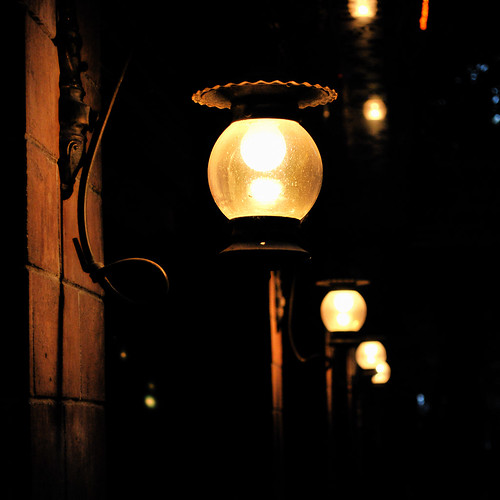
\includegraphics[draft]{imageNight.png}
			\caption{Изобр. категории низкая освещенность.}
			\label{ris:experimcoded}
		\end{minipage}
	\end{center}
\end{figure}

\subsubsection{Видео}
Данные необходимые для исследования видео последовательность были взяты из открытой базы данных  YouTube-8M.


Ниже приведены кадры из видео каждой категории.
\begin{figure}[H]
	\begin{center}
		\begin{minipage}[h]{0.5\linewidth}
			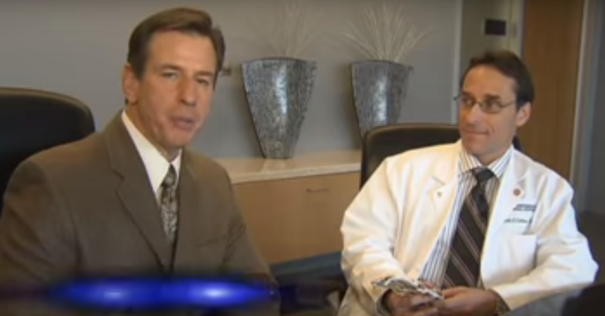
\includegraphics[draft]{videoPerson.png}
			\caption{Видео категории человек.} %% подпись к рисунку
			\label{img:imPerson} %% метка рисунка для ссылки на него
		\end{minipage}
		\hfill 
		\begin{minipage}[h]{0.5\linewidth}
			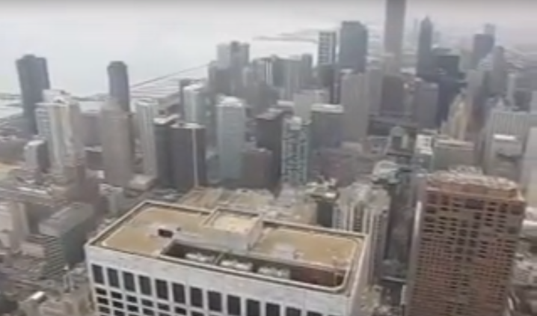
\includegraphics[draft]{videoArchitecture.png}
			\caption{Видео категории архитектура.}
			\label{img:imArchitecture}
		\end{minipage}
		\hfill 
		\begin{minipage}[h]{0.5\linewidth}
			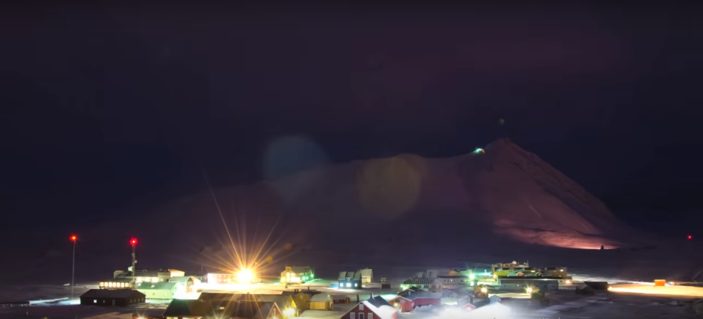
\includegraphics[draft]{videoNight.png}
			\caption{Видео категории низкая освещенность.}
			\label{ris:experimcoded}
		\end{minipage}
	\end{center}
\end{figure}
\subsection{Схема программы}
Работу реализованной программы можно описать следующим образом. На вход программы подаются данные (видео или изображение). Далее накладывается гауссовский шум. После проводится шумоподавления различными алгоритмами с различными параметрами. В итоге выбирается алгоритм, которые показал наибольшие показатели PSNR и SSIM. Для каждой категории берутся максимальные и средние значения значения PSNR, SSIM.
\begin{figure}[H]
	\center{\includegraphics[draft]{programm.png}}
	\caption{Схема итоговой программы}
\end{figure}
\subsection{Результаты исследования}
Исследование разбито на две части. В первой части для каждого алгоритма подбираются оптимальные параметры, которые дают максимальной значение PSNR или SSIM для определенного типа изображения или видео. Исходя уже из полученных результатов будут сравниваться между собой все алгоритмы.

